\section{Sensitivity Analysis}
\label{a:sensitivity-analysis}

The sensitivity analysis was carried out by performing a feature scoring analysis. Feature scoring was chosen, as also described in section \ref{ss:sensitivity-analysis}, because while still using the SOBOL sampling method, it has lower computational requirements \cite{jaxa-rozen_tree-based_2018}. The results from this can be seen in the figures below. 

\begin{figure}[h!]
    \centering
    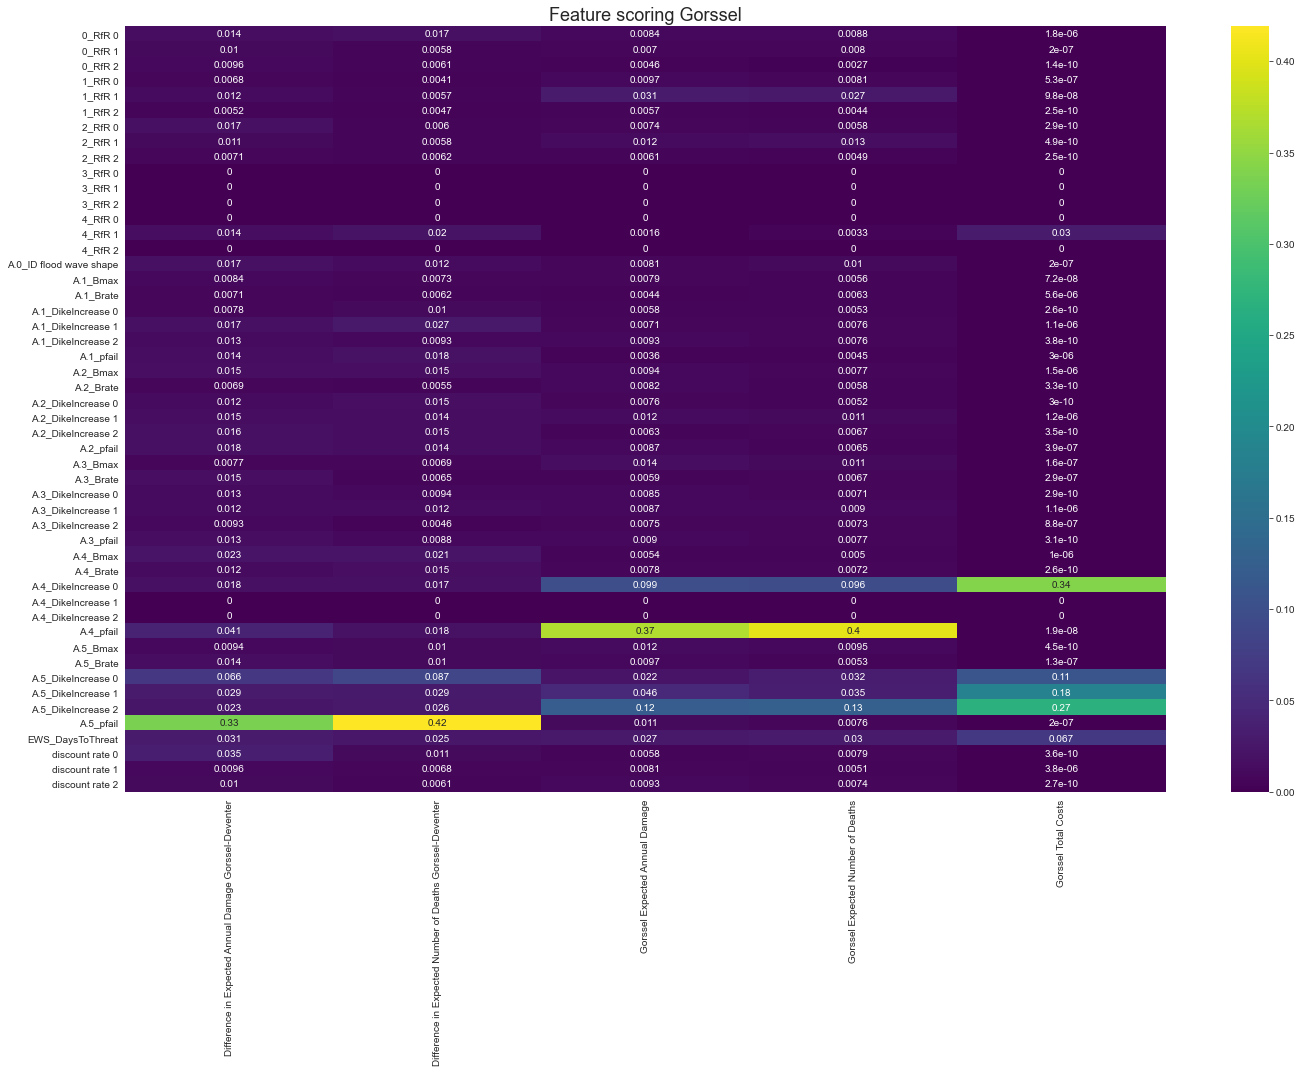
\includegraphics[width=\textwidth]{report/figures/results/Feature_scoring_Gorssel_100scen.png}
    \caption{The results from feature scoring for the sensitivity analysis of Gorssel}
    \label{fig:feat-scor-g}
\end{figure}

\begin{figure}[h!]
    \centering
    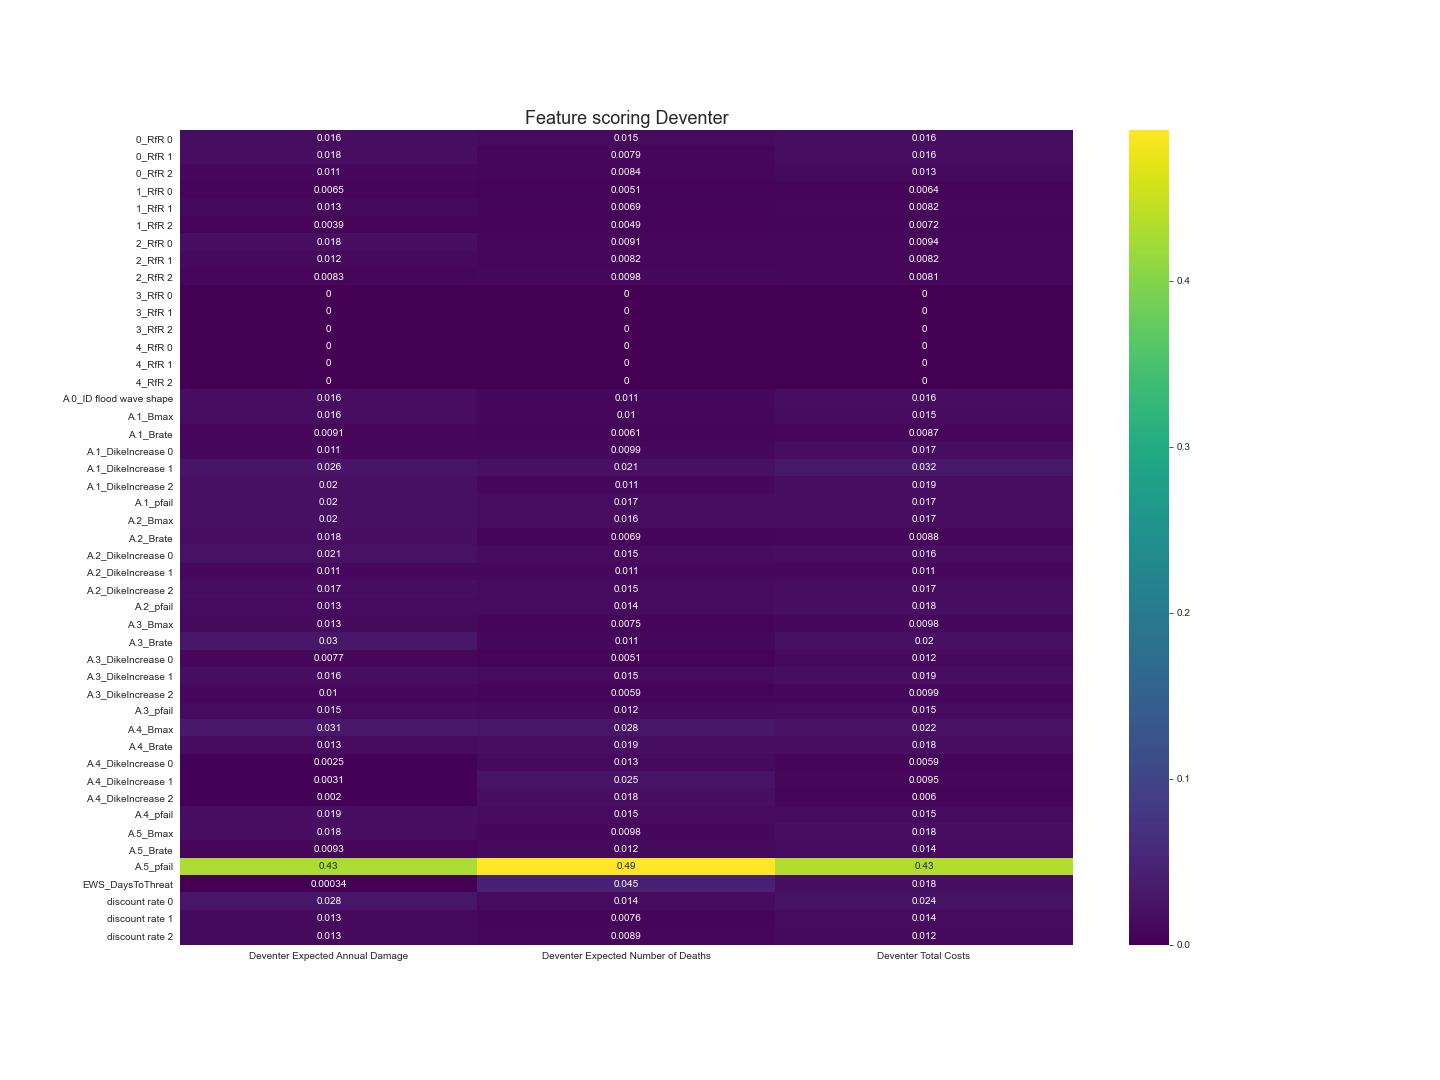
\includegraphics[width=\textwidth]{report/figures/results/Feature_scoring_Deventer_100scen.png}
    \caption{The results from feature scoring for the sensitivity analysis of Deventer}
    \label{fig:feat-scor-d}
\end{figure}

\begin{figure}[h!]
    \centering
    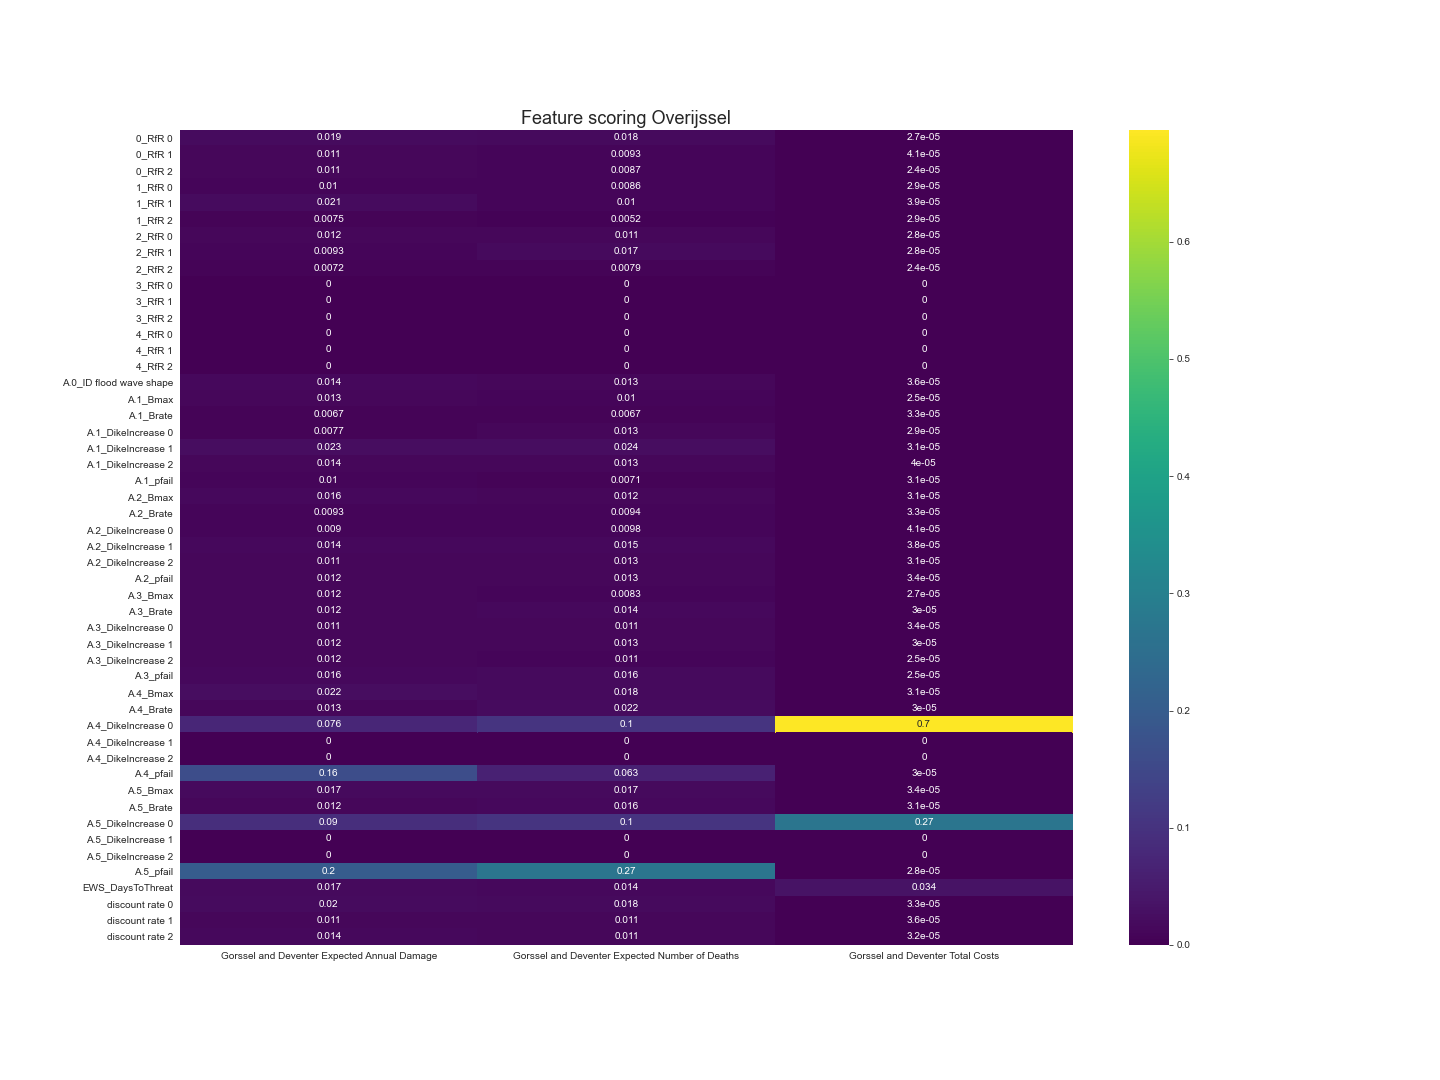
\includegraphics[width=\textwidth]{report/figures/results/Feature_scoring_Overijssel_100scen.png}
    \caption{The results from feature scoring for the sensitivity analysis of Overijssel}
    \label{fig:feat-scor-o}
\end{figure}

\begin{figure}[h!]
    \centering
    \includegraphics[width=\textwidth]{report/figures/results/}
    \caption{The results from feature scoring for the sensitivity analysis of Gorssel}
    \label{fig:feat-scor-g}
\end{figure}

\begin{figure}[h!]
    \centering
    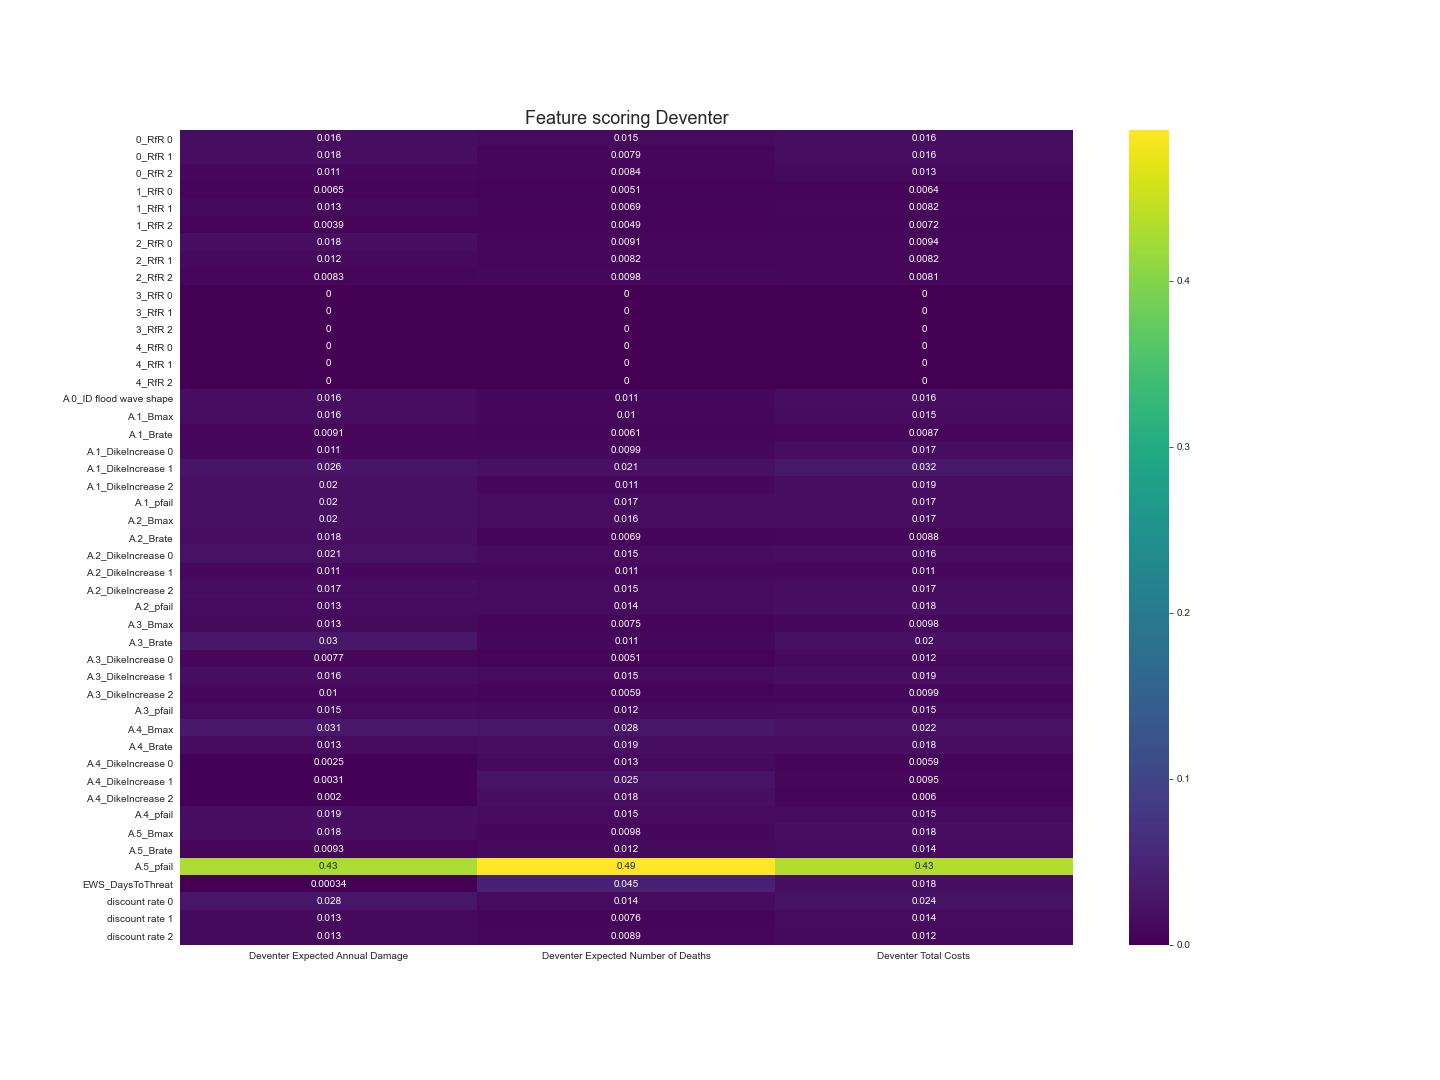
\includegraphics[width=\textwidth]{report/figures/results/Feature_scoring_Deventer_100scen.png}
    \caption{The results from feature scoring for the sensitivity analysis of Deventer}
    \label{fig:feat-scor-d}
\end{figure}

\begin{figure}[h!]
    \centering
    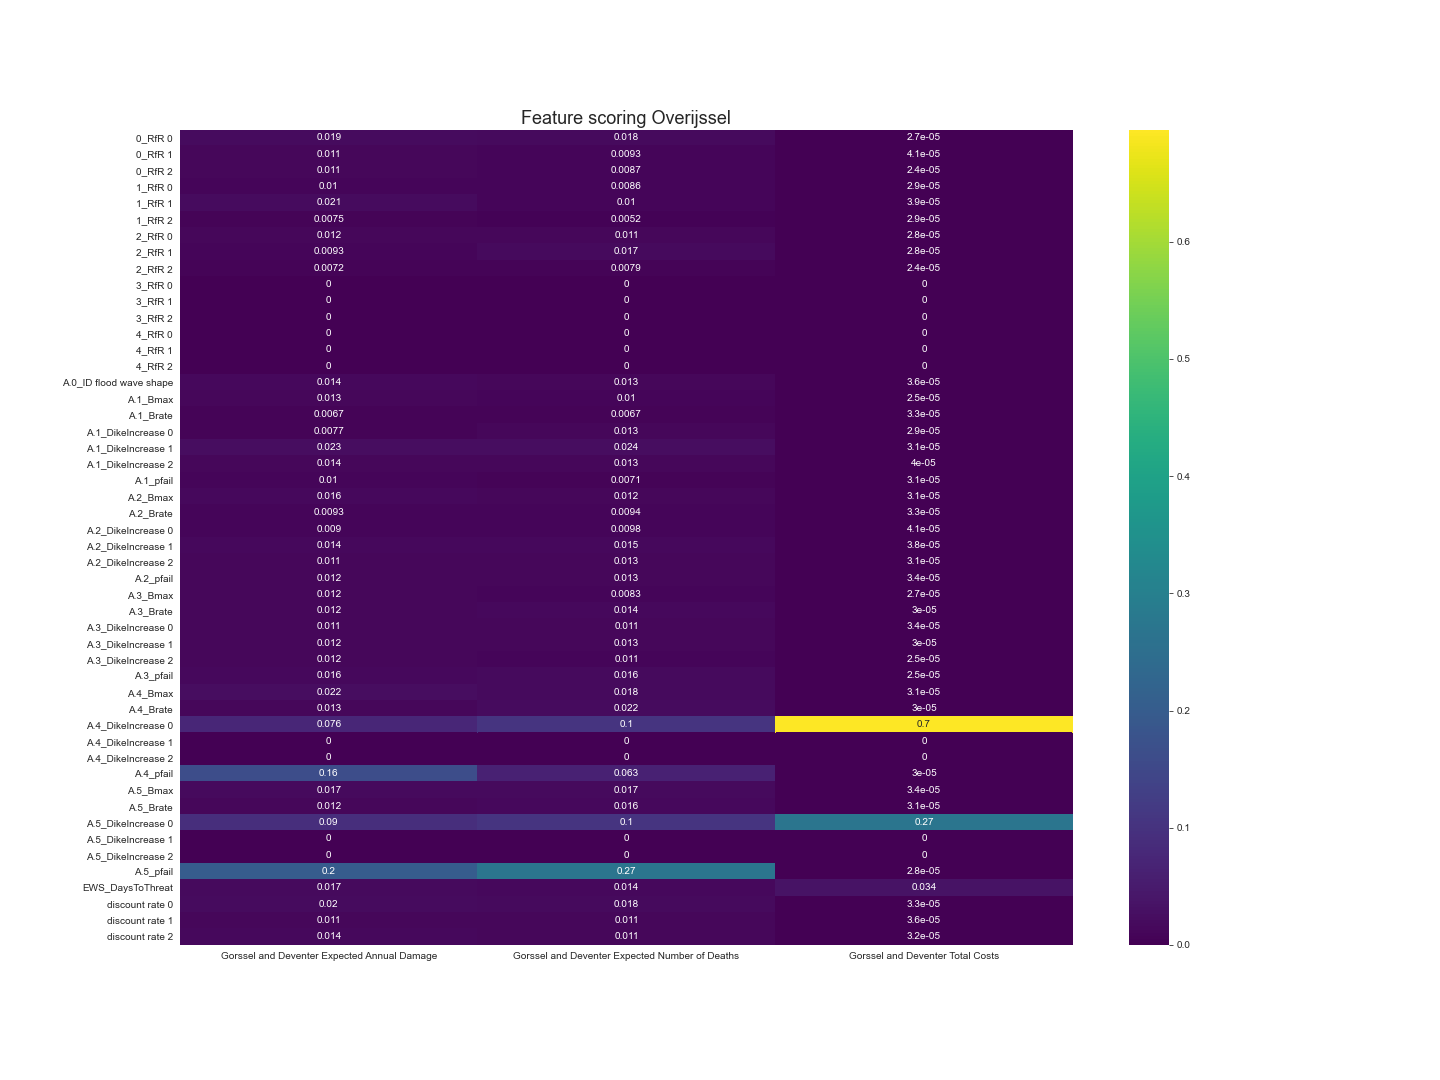
\includegraphics[width=\textwidth]{report/figures/results/Feature_scoring_Overijssel_100scen.png}
    \caption{The results from feature scoring for the sensitivity analysis of Overijssel}
    \label{fig:feat-scor-o}
\end{figure}